\documentclass{article}%
\usepackage[T1]{fontenc}%
\usepackage[utf8]{inputenc}%
\usepackage{lmodern}%
\usepackage{textcomp}%
\usepackage{lastpage}%
\usepackage[head=40pt,margin=0.5in,bottom=0.6in]{geometry}%
\usepackage{graphicx}%
%
\title{\textbf{Ligia Bolívar: Aceptar la ayuda humanitaria está en manos del gobierno}}%
\author{EL NACIONAL WEB}%
\date{28/09/2018}%
%
\begin{document}%
\normalsize%
\maketitle%
\textbf{URL: }%
http://www.el{-}nacional.com/noticias/politica/ligia{-}bolivar{-}aceptar{-}ayuda{-}humanitaria{-}esta{-}manos{-}del{-}gobierno\_253561\newline%
%
\textbf{Periodico: }%
EN, %
ID: %
253561, %
Seccion: %
Política\newline%
%
\textbf{Palabras Claves: }%
Política\newline%
%
\textbf{Derecho: }%
18%
, Otros Derechos: %
5%
, Sub Derechos: %
NO\_TIENE%
\newline%
%
\textbf{EP: }%
NO\newline%
\newline%
%
\textbf{\textit{La directora del Centro de Derechos Humanos de la Universidad Católica Andrés Bello indicó que la ONU no puede obligar al Estado venezolano a aceptar apoyo internacional}}%
\newline%
\newline%
%
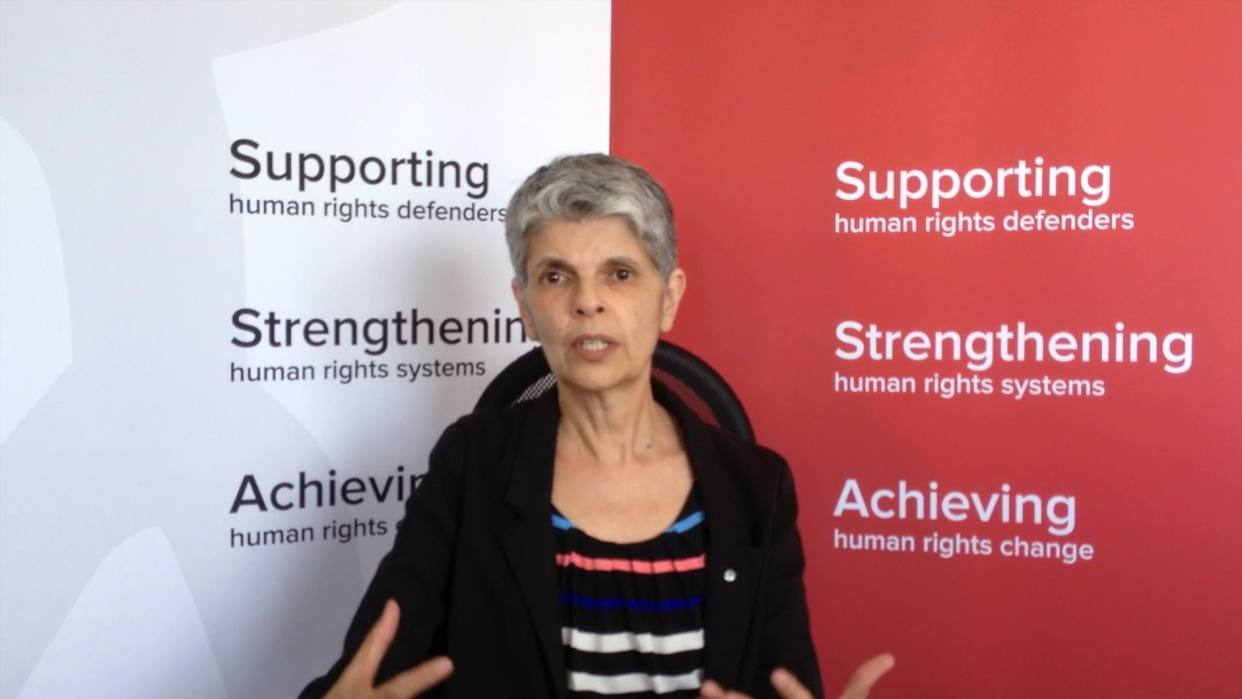
\includegraphics[width=300px]{121.jpg}%
\newline%
%
Ligia Bolívar, directora del Centro de Derechos Humanos de la Universidad Católica Andrés Bello, señaló este viernes que la Organización de las Naciones Unidas (ONU) no tiene la fuerza coercitiva para obligar al Estado venezolano a recibir una ayuda humanitaria.%
\newline%
%
Durante una entrevista ofrecida en TVVenezuela Noticias, Bolívar indicó que aunque el Consejo de Derechos Humanos de la ONU~aprobó la resolución sobre la crisis humanitaria en Venezuela, son las autoridades venezolanas las que pueden abrir las puertas para que la ayuda~se lleve a cabo.%
\newline%
%
"Venezuela vive, desde hace muchos años atrás, en una crisis de desobediencia, de rebeldía, de desacato abierto a la comunidad internacional. Esa resolución es importante porque es la primera vez que la comunidad internacional se pone de acuerdo y dice: Venezuela tiene que abrir las puertas a la ayuda humanitaria y tiene que abrir las puertas de verificacion por parte de las Naciones Unidas. Ahora, que venezuela cumpla o no, ya no está en manos del consejo, está en manos de las autoridades venezolanas", agregó Bolívar.%
\newline%
%
\end{document}